\chapter{Problems and Future Work}\label{prbftr}
This chapter focuses on problems and future work. Section \ref{prblms} presents some flaws in the prediction results, along with the corresponding possible solutions. Section \ref{ftrwrk} shows the future direction of our work.

\section{Problems}\label{prblms}
In this section, two existed problems in the prediction result are illustrated, and for each problem, we propose potential solutions respectively. Subsection \ref{outres} shows the resolution problem resulting in the inaccurate prediction and subsection \ref{flsvtx} shows the problem of the false vertex.

\subsection{Output Resolution}\label{outres}
We know that the output grid for a single vertex has the resolution 28$\times$28, and the resolution of input images of PolygonRNN is 224$\times$224. Thus, a single pixel in the output grid corresponds to an area of 8$\times$8 in the original image. This will result in blurs on the feature map and loss of details, therefore outputting inaccurate vertices. Figure \ref{fig:resprob} gives some examples, where the prediction of those round or semicircular buildings in Zurich is very inaccurate, and the prediction of buildings with small bulges in Chicago cannot well match the edges of buildings in the original image. Please zoom in for more details.

\begin{figure}[!h]
	\centering
	\subbottom[resolution problem in the dataset of Zurich\label{fig:resprobzh}]{
		\includegraphics[width=\figfigfigfig\textwidth]{5-00-0.png}
		\includegraphics[width=\figfigfigfig\textwidth]{5-00-1.png}
		\includegraphics[width=\figfigfigfig\textwidth]{5-00-2.png}
		\includegraphics[width=\figfigfigfig\textwidth]{5-00-3.png}
	}
	\subbottom[resolution problem in the dataset of Chicago\label{fig:resprobch}]{
		\includegraphics[width=\figfigfigfig\textwidth]{5-00-4.png}
		\includegraphics[width=\figfigfigfig\textwidth]{5-00-5.png}
		\includegraphics[width=\figfigfigfig\textwidth]{5-00-6.png}
		\includegraphics[width=\figfigfigfig\textwidth]{5-00-7.png}
	}
    \caption[Examples of resolution problem in Zurich and Chicago]{Examples of resolution problem in Zurich and Chicago.}
	\label{fig:resprob}
\end{figure}


The possible solution is to increase the resolution of the output grid, and to extract features from relatively shallow levels. However, these shallow layers may not have much semantic information, which may further have a negative effect on the prediction accuracy of RNN part. In addition, because of the existence of FC layer at the end of the output of RNN part, the number of its weights would increase at the fourth power, i.e. $\Theta(w^2h^2)$. For example, currently, the FC layer has $(28^2)^2 = $ 614,656 weights, if we increase the resolution of the output grid to 56$\times$56, the number of weights would be $(56^2)^2 = $ 9,834,496, 16 times the original. The explosively increasing parameters can make the entire network more difficult to train, and meanwhile, it would also greatly increase the time and space (storage) consumption. Therefore, the conclusion is that if the resolution is increased, we would better adapt the network structure to meet the requirement.

\subsection{False Vertex}\label{flsvtx}
Actually, after the introduction of beam search algorithm, the false vertex problem has been solved a lot and the prediction is greatly improved (see table \ref{tab:evalmodin}), but there are still some in the results, which are shown in figure \ref{fig:flsprob}.

In the dataset of Zurich, the false vertex issue is mainly focused on the order of the vertices. For example, the two adjacent vertices that should be sequential are predicted to be in reverse order, thus the original ``L" shape building would show a ``zigzag" shape (see figure \ref{fig:flsprobzh}).

As for the dataset of Chicago, many buildings are predicted to have bulges and produce sharp corners (see figure \ref{fig:flsprobch}). We think this is mainly influenced by the shadows of the buildings.

\begin{figure}[!h]
	\centering
	\subbottom[false vertex problem in the dataset of Zurich\label{fig:flsprobzh}]{
		\includegraphics[width=\figfigfigfig\textwidth]{5-01-0.png}
		\includegraphics[width=\figfigfigfig\textwidth]{5-01-1.png}
		\includegraphics[width=\figfigfigfig\textwidth]{5-01-2.png}
		\includegraphics[width=\figfigfigfig\textwidth]{5-01-3.png}
	}
	\subbottom[false vertex problem in the dataset of Chicago\label{fig:flsprobch}]{
		\includegraphics[width=\figfigfigfig\textwidth]{5-01-4.png}
		\includegraphics[width=\figfigfigfig\textwidth]{5-01-5.png}
		\includegraphics[width=\figfigfigfig\textwidth]{5-01-6.png}
		\includegraphics[width=\figfigfigfig\textwidth]{5-01-7.png}
	}
    \caption[Examples of false vertex problem in Zurich and Chicago]{Examples of false vertex problem in Zurich and Chicago.}
	\label{fig:flsprob}
\end{figure}


The possible solution comes from the point of view of geometry, penalizing the angles with strange degrees in the polygon (e.g. acute angles). Figure \ref{fig:agldstb} shows the polygon interior angle degree distribution in the dataset of Zurich and Chicago.

\begin{figure}[!h]
	\centering
	\subbottom[angle distribution in Zurich\label{fig:agldstbzurich}]{
		\includegraphics[width=\figfig\textwidth]{5-02-0.pdf}
	}
	\subbottom[angle distribution in Chicago\label{fig:agldstbchicago}]{
		\includegraphics[width=\figfig\textwidth]{5-02-1.pdf}
	}
    \caption[Polygon interior angle distribution]{Polygon interior angle distribution.}
	\label{fig:agldstb}
\end{figure}

From figure \ref{fig:agldstbchicago} we can see that in Chicago, most angles are at $90^\circ$ or $270^\circ$, indicating that most of them are right angles, which is easier for a machine to learn. This is also the reason why the dataset of Chicago gets a higher performance. In Zurich's figure \ref{fig:agldstbzurich}, although most angles are around $90^\circ$ or $270^\circ$, they have certain deviations about $\pm20^\circ$. Also, there is a peak near $180^\circ$ in figure \ref{fig:agldstbzurich}, which means that there are many three-point collinearities in the dataset of Zurich.

In practice of penalizing the angle degree of the polygon, when doing the probability computation of the next vertex, we can use the distribution of the angle $\theta$ as a priori to guide the prediction or make a manual intervention. For example, we can simply replace $P(v_t \mid v_{t-1}, v_{t-2})$ in equation \ref{eq:vnext} with $P(v_t \mid v_{t-1}, v_{t-2}, \theta)$. This requires the function $F$ to take $\theta$ as input, which also requires a change of the network structure in order to feed this prior in.

\section{Future Work}\label{ftrwrk}
In this section, several future directions of our work are presented, such as the possible direction of roads segmentation, the improvement of the dataset, the methods that are helpful for training and the possible extensions of the model.

\paragraph{Segmentation of Roads}
At present, our thesis project does not include road segmentation. This is because roads usually cannot be represented as polygons. However, we still hope to add this kind of segmentation in the future, so that the geometrical instance segmentation in aerial images can become complete, and we can also further learn the geometrical layout of the city from aerial images. The basic idea for roads segmentation is to convert roads into centerlines and intersections. Figure \ref{fig:pararoad} shows an example.

\begin{figure}[!h]
	\centering
	\includegraphics[width=\figfi\textwidth]{5-04.pdf}
    \caption[A possible approach of road parameterization]{A possible approach of road parameterization.}
	\label{fig:pararoad}
\end{figure}

Actually, in Mask R-CNN \cite{maskrcnn}, the part of human posture detection is exactly doing this, where a person is structured as several keypoints with edges connecting them. Figure \ref{fig:posdet} shows some human posture detection results of Mask R-CNN.

\begin{figure}[!h]
	\centering
	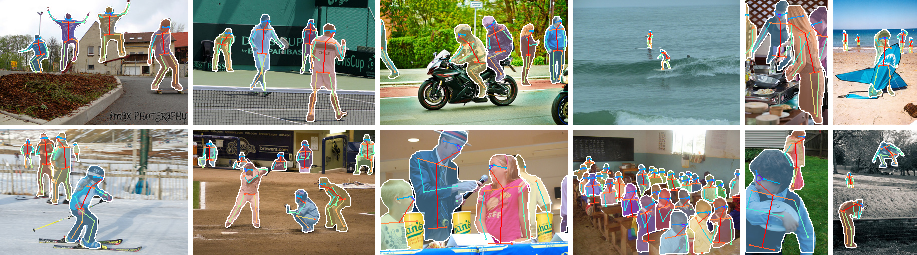
\includegraphics[width=\fig\textwidth]{5-03.pdf}
    \caption[Human posture detection in Mask R-CNN]{Human posture detection in Mask R-CNN. Image copyright owned by \cite{maskrcnn}.}
	\label{fig:posdet}
\end{figure}

However, it is difficult to apply this method to our project, because the road is different from the human body, the number of keypoints of roads in each image is not fixed. That is the biggest obstacle to structurize roads.

\paragraph{Ground Truth Correction}
Subsection \ref{adjust} has already introduced a method to correct ground truth. However, there are still some image-polygon pairs inaccurate, especially for those adjacent buildings (see figure \ref{fig:egshi3}). We hope that the dataset can be collected from a single source, so that the polygons and the buildings are more likely to match each other. As for the adjacent buildings, it is difficult for us to merge their polygons into a single one. Thus, we hope polygons of buildings instead of houses can be provided.

\paragraph{RoIAlign Implementation}
Subsection \ref{algmod} has already introduced the hybrid version with RoIAlign of \modelnameshort. We hope that in the future, this kind of version can be implemented and tested. In theory, it can speed up both the training and prediction phases.

\paragraph{Training Method}
Our model does not use pre-trained VGG-16 during training, neither as an initializer nor as fixed weights. In the future we may apply the pre-trained VGG-16 to our model's training. Besides, we hope that the alternating training method can be introduced, of which the main idea is to train the subnetworks separately, then train them together and fine-tune the whole model. For more details about this kind of training, please refer to the Fast R-CNN paper \cite{fasterrcnn}.

\paragraph{Model Generalization}
In fact, our model can be applied not only to the geometrical instance segmentation in the aerial images, but also to other kinds of images which contain multiple objects. We hope that our model \modelnameshort\ can be generalized to other fields and we can compare the performance under different dataset.

